\documentclass{article}
\usepackage[cm]{fullpage} %very small margins (around 1.5cm)
\usepackage{enumitem} %remove vertical space in itemize with: [noitemsep,nolistsep]
\usepackage{multicol} %use \begin{multicols}{#} for # columns 
\usepackage{graphicx} %use \includegraphics[scale=1.00]{file.jpg} for images
\usepackage{color}
\usepackage[usenames,dvipsnames]{xcolor}
\usepackage{lastpage} %page x of y with: \cfoot{\thepage{} of \pageref{LastPage}}
\usepackage{fancyhdr} % also needed for footers
\usepackage{minted} %use \begin{minted}[mathescape,linenos,numbersep=5pt,gobble=0,framesep=2mm]{c++}

\fancyhead{}
\fancyfoot{}
\lfoot{\textcolor{gray}{M.Bysiek R.Lojek S.Peryt}}
\cfoot{page \thepage{} of \pageref{LastPage}}
\rfoot{\textcolor{gray}{VaDoR}}
\pagestyle{fancy}
\renewcommand{\headrulewidth}{0pt}
\renewcommand{\footrulewidth}{0pt}

\begin{document}

\title{VAnishing DOmino pRoblem - VaDoR}
\author{Mateusz Bysiek, Radoslaw Lojek, Stanislaw Peryt; Computer Science, MiNI, WUT}
\date{17 October 2012}
\maketitle

\begin{multicols}{2}
\begin{flushleft}

\includegraphics[scale=0.60]{logo_pw.jpg}
\end{flushleft}
\begin{flushright}

\includegraphics[scale=0.25]{logo_mini.png}
\end{flushright}
\end{multicols}

\tableofcontents

\pagebreak[4]

\section{Problem description}
Vanishing domino problem. Full definition is available in the document provided by laboratories
supervisor. From now on, the problem will be referred to as VaDoR.

\section{Estimation of complexity}
\subsection{Number of states}
Let us assume that we have a set of $n$ domino pieces that are arranged on a board. Then, 
let us assume that we are taking away pieces from the board, one at a time. If we consider each 
state after removing a piece, how many different states do we have? For a given state, for each piece, 
we have a choice: the piece either is on the board, or it is not. In total we have $2$ possible scenarios
for one piece, and $n$ pieces, which gives us exactly $2^n$ different states.

\subsection{Relations between the states}
We can construct a following directed acyclic graph (DAG) $G$:
\begin{enumerate}[noitemsep,nolistsep]
  \item each vertex $V$ represents a state (configuration of pieces on the board)
  \item each directed edge $E$ represents the relation between states. Edges 
  are positioned in such way, that start point is at state $V_1$, and such that 
  the end point of the edge is connected to the state $V_2$ that can be obtained 
  directly from state $V_1$ by removing one domino piece from the board.
\end{enumerate}

\subsection{Estimation}
Having a DAG $G$, the domino problem is equivalent to finding the longest path of DAG. 
Unfortunately, graph has to be constructed at runtime, and that takes time. 

Since, for each state, the calculation of related states will be performed (and there are $2^n$ states in total)
I estimate the complexity of algorithm as exponential. I also informally classify 
this problem as NP. After the DAG is constructed, by finding its longest path, an optimal 
solution is obtained.

My estimations indicate that calculation of related states for a given single 
state takes polynomial time. Finding the longest path in DAG takes linear time. 
Therefore, the total complexity of the accurate algorithm should be roughly $ 2^n * n^2 + n $

\section{Description of the accurate algorithm}
\subsection{Input}
XML file.
\begin{minted}[linenos,numbersep=5pt]{xml}
<domino_board width="5" height="4">
    <piece x="0" y="0" orientation="vertical" value1="2" value2="1" />
    <piece x="0" y="2" orientation="vertical" value1="3" value2="2" />
    <piece x="1" y="0" orientation="horizontal" value1="1" value2="0" />
    <piece x="1" y="1" orientation="vertical" value1="3" value2="0" />
    <piece x="1" y="3" orientation="horizontal" value1="0" value2="0" />
    <piece x="2" y="1" orientation="vertical" value1="1" value2="1" />
    <piece x="3" y="0" orientation="horizontal" value1="3" value2="3" />
    <piece x="3" y="1" orientation="vertical" value1="0" value2="2" />
    <piece x="3" y="3" orientation="horizontal" value1="2" value2="2" />
    <piece x="4" y="1" orientation="vertical" value1="4" value2="4" />
</domino_board>
\end{minted}

\pagebreak[4]

Description of the \verb|piece| tag:
\begin{itemize}[noitemsep,nolistsep]
  \item x - coordinate, from zero, increasing from the right to the left side of the board
  \item y - coordinate, from zero, increasing from the top to the bottom side of the board
  \item orientation:
	\begin{itemize}[noitemsep,nolistsep]
  	\item \emph{horizontal} - the piece starts at $(x,y)$ and ends at $(x+1,y)$
  	\item \emph{vertical} - the piece starts at $(x,y)$ and ends at $(x,y+1)$
	\end{itemize}
  \item value1 - value of the beginning of the piece i.e. value at $(x,y)$
  \item value2 - value of the end of the piece i.e. location depends on the orientation
\end{itemize}

\vspace{7pt}

If a tag \verb|removed_pieces| is present inside the \verb|domino_board| tag, it is ignored. If an
attribute \verb|order| is attached to the \verb|piece| tag, it is also ignored. That way the output file 
can be used as an input, and pieces can be rearanged and put back on the board using a text editor, without
worrying about problems with parsing.

\subsection{Output}
Another XML file.

\begin{minted}[linenos,numbersep=5pt]{xml}
<domino_board width="5" height="4">
    <piece x="0" y="0" orientation="vertical" value1="2" value2="1" />
    <piece x="0" y="2" orientation="vertical" value1="3" value2="2" />
    <piece x="3" y="0" orientation="horizontal" value1="3" value2="3" />
    <piece x="4" y="1" orientation="vertical" value1="4" value2="4" />
    <removed_pieces>
       <piece order="0" x="1" y="0" orientation="horizontal" value1="1" value2="0" />
       <piece order="1" x="1" y="1" orientation="vertical" value1="3" value2="0" />
       <piece order="2" x="2" y="1" orientation="vertical" value1="1" value2="1" />
       <piece order="3" x="3" y="1" orientation="vertical" value1="0" value2="2" />
       <piece order="4" x="1" y="3" orientation="horizontal" value1="0" value2="0" />
       <piece order="5" x="3" y="3" orientation="horizontal" value1="2" value2="2" />
    </removed_pieces>
</domino_board>
\end{minted}

It is an extension of an input format. Program will be designed in such a way, that output from the program 
can be used again as an input (as it is described in ``Input'' section).

\vspace{7pt}

Description of extension the \verb|piece| tag:
\begin{itemize}[noitemsep,nolistsep]
  \item order - number, from zero, increasing in order in which the pieces were removed from the board
\end{itemize}

\vspace{7pt}

The \verb|removed_pieces| tag contains all of the pieces that were removed from the board, with complete 
information about their origin. 

\subsection{Class variables}
Main class of the program is called domino\_problem.

Rough list of fields of the class:
\begin{minted}[linenos,numbersep=5pt]{c++}
/* elements_t is a list of domino pieces */
   // collection of pieces
   elements_t elements;
   size_t width;
   size_t height;
   // collection of halves of pieces that come from 'elements' field
   board_t board;
   // pieces currently on the board
   elements_t on_board;
   // possible to remove in the next turn
   elements_t possible;
   // not longer on board, removed in the previous turns
   elements_t removed;
   // algorithm does not know anything about these pieces
   elements_t unresolved;
   // possible to remove if other pieces are placed right
   elements_t checked;
   // impossible to remove due to size of the board
   elements_t invalid;
\end{minted}

There is also a supporting variable, graph, which stores data about every state analyzed by the
algorithm.
\begin{minted}[mathescape,linenos,numbersep=5pt,gobble=0,framesep=2mm]{c++}
   graph_t graph
\end{minted}

\subsection{Algorithm}
Because of large number of loops involved in the algorithm, 
I will not provide pseudocode, and will write down 
a description of instructions instead.

\begin{enumerate}[noitemsep,nolistsep]
   \item Input data is read: width and height.
   \item All pieces present on board are stored into 'elements' field
   this list does not change with time
   \item 'board' is generated for convienience.
   \item 'elements' are copied into other lists: 'on\_board' and 'unresolved'
   \item 'unresolved' are partitioned into 'checked' and 'invalid'
   \item add current problem to the graph
   \item CHECKING: each piece from 'checked' is examined, and if it can be removed 
   from the board it is copied to 'possible'
   \item for each 'possible' piece, new object of class domino\_problem is created
   via copy constructor
   \begin{enumerate}[noitemsep,nolistsep]
	   \item from each copy of current domino\_problem, the corresponding piece of 'possible'
	   is moved to 'removed', and the same piece is deleted from 'checked', 'on\_board' 
	   and 'board'.
	   \item all lists of 'possible' from current domino\_problem copies are cleared
	   \item add all copies to the graph with exception of those that already exist
	   in the graph, because removing first piece A and then B gives the same resulting state 
	   as removing first piece B and then A. Calculating all possibilities with duplicates would
	   result in factorial complexity of the algorithm ($n!$).
	   \item connect current problem to all of the copies
	   \item for each copy, perform all steps starting from CHECKING
	\end{enumerate}
	\item after the graph is constructed, find the longest path, starting from 
   initial domino\_problem.
\end{enumerate}

\section{Description of the approximate algorithms}

\subsection{By Mateusz Bysiek}
\subsubsection{Input}
The same as in case of accurate algorithm.
\subsubsection{Class variables and algorithm}
Development of approximations of NP problems is usually a consequence 
of deep understanding of the problem, and extensive experience in solving it using
some kind of accurate algorithm. Without them, randomization can be used.
My approximate algorithm is a polynomial time random algorithm.

It uses the same data structures as mentioned in the accurate algorithm, but it simply randomly
chooses one possible option and tries to resolve it (in step 8. it does not have any loop).
If a dead end is reached, the algorithm ends and returns so-far-calculated path.

\pagebreak[4]

\subsection{by Stanislaw Peryt}

\subsubsection{Input Data}
collection of domino pieces from input file
\subsubsection{Description and Class Variables}
This algorithm is based on the idea of Greedy algorithms. I assume some additional classification
which is done only once for each element. For classification purposes each dominoPiece should
contain some additional fields:

\begin{minted}[linenos,numbersep=5pt]{c++}
boolean isIndependent; //can be removed even from empty board, so it does not have to 
   // be removed immediately
boolean canBeRemoved; //initially false. Changes to true, when fulfills removal conditions
list<waitingFor>; // list of pieces for which it is waiting;
list<waitForMe>; // list of pieces waiting for it;
\end{minted}

I decided to add this classification, because in greedy strategy, we could remove pieces immediately
when they fulfill removal requirements. But it may happen, that there are some pieces, for which
pieces we already removed are necessary to fulfill removal requirements. When we have this
classification based on scopes of domino pieces, we can wait with removing, and eliminate at least
some of those situations described above, providing better local optimal choices.

For this algorithm we also need:
board � contains all domino pieces that have remained on the board
roots � contains possible starting pieces, i.e. containing zero
neighbors � contains domino pieces, which are neighbors of deleted piece, i.e. pieces alongside empty fields
\subsubsection{Algorithm}
\begin{enumerate}[noitemsep,nolistsep]
   \item Create board from input
   \item Find possible roots and assign them to neighbors
   \item for each dominoPiece in board assign scopes and waiting property
   \begin{enumerate}[noitemsep,nolistsep]
      \item determine scopes based on numbers given on dominoPiece
      \item determine dominoPieces on scopes and assign them to the waitForMe list
      \item tell those pieces to assign this dominoPiece on their waitingFor list
   \end{enumerate}
   \item stop=false;
   \item while(!stop)\{
   \begin{itemize}[noitemsep,nolistsep]
     \item for each dominoPiece in neighbors\{
         \begin{enumerate}[noitemsep,nolistsep]
            \item if dominoPiece can be removed \{
            \begin{enumerate}[noitemsep,nolistsep]
               \item if (domino Piece isIndependent) and (list of pieces it is waiting for is not empty) \{ \\
                  wait with removal; \\
               \}
               \item else
                  remove it(from neighbors and board) and tell waiting pieces, if there were any waiting
                  for this piece, that it does not need waiting any more. (i.e. delete piece from waiting
                  list)
            \end{enumerate}
            \}
         \end{enumerate}
         \} \\
         determine new neighbors into temp (each removed piece can produce at most 6 new neighbors)
     \item if temp equals neighbors\{
         \begin{itemize}[noitemsep,nolistsep]
            \item check if (something can be removed): remove first;
            \item else stop=true;
         \end{itemize}
         \}
     \item else neighbors=temp;
   \end{itemize}
   \}
   \item calculate score
\end{enumerate}
\subsubsection{Estimation of complexity}
Partial Complexities:

$n$-complexity of classification

$n^2$-complexity of part at �while(!stop) loop�

In order to associate attributes for classification we need to iterate once through whole collection
which is of size n. Then in the while loop we are trying to remove pieces. In worst case we delete
only one piece in one iteration which gives us at most n runs of while and inside while loop, we
iterate through neighbors collection which is always smaller than n, but it is n dependent.
Therefore for each n, algorithm executes number of operations proportional to n, which gives us
quadratic time complexity.

Final worst case complexity : $n^2 + n$

\subsection{by Radoslaw Lojek}

\subsubsection{Introduction}
The solution I have designed is the most intuitive and straight forward algorithm. It checks all
possible elements along its way. If a domino piece satisfies necessary conditions of being removed,
it is thrown away from a board of elements. The operation is repeated for all consecutive elements
until nothing can't be removed, or the domino board is empty.


\subsubsection{Algorithm Pseudo-Code}
The algorithm takes as a parameters two dimensional array of elements and its vertical and
horizontal size. Returns elements that were removed during the calculations. Below algorithm is
simple, since it does not involve more complicated concepts such as Artificial Intelligence or
complex graph algorithms.
\\
\begin{minted}[linenos,numbersep=5pt]{c++}
List<dominoPiece> solveDominoProblem(dominoField **board, int dimX, int dimY){
   List<dominoPiece> result_list;
   int iterPiecesRemoved = 1;
   
   while iterPiecesRemoved != 0 {
      iterPiecesRemoved = 0;
      for i = 0 to dimX {
         for j = 0 to dimY {
            if !isEmpty(board,i,j) and isElemRemovable(board, dimX, dimY, i, j){ 
               result_list.add( removePiece(board,i,j) );
               iterPiecesRemoved = iterPiecesRemoved + 1;
            }
         }
      }
   }
   return result_list;
}
\end{minted}

%\begin{wrapfigure}{r}{0.3\textwidth}
%  \vspace{-30pt}
  \begin{center}
    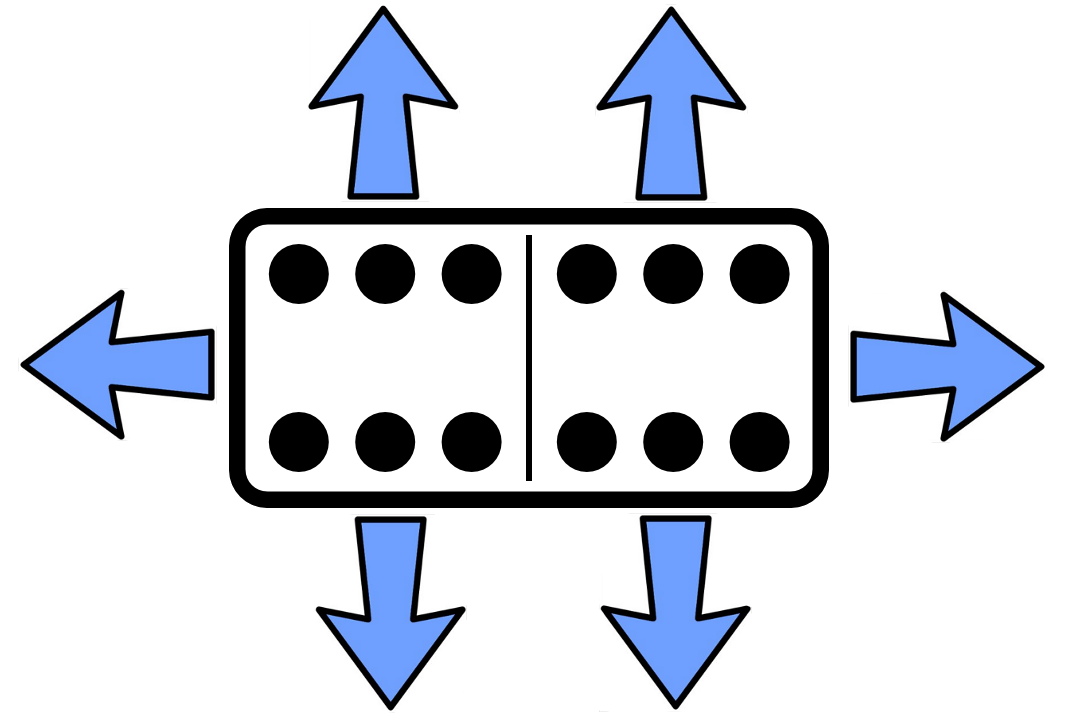
\includegraphics[width=0.2\textwidth]{dirPiece.png}
  \end{center}
 % \vspace{-20pt}
%\end{wrapfigure}

I will let myself omit pseudo code of functions used above. Just briefly explain how isElemRemovable
will work: depending on the location of a 'twinField' of a single piece, function counts the number
of empty fields in each possible direction (as depicted on the right). Once the directions are
counted, function checks if they meet requirements for the piece to be removed - if it does, returns
true or false otherwise.

\subsubsection{Time complexity}
Time complexity of the considered algorithm is \textit{$n^2$}, since we go in each iteration 
through all possible domino fields \textit{n} times. Each iteration is repeated in worst case
\textit{1/2*n} times, because may occur situation in which only one domino element (two fields)
disappears in one \textit{while} loop iteration.

\subsubsection{Example}

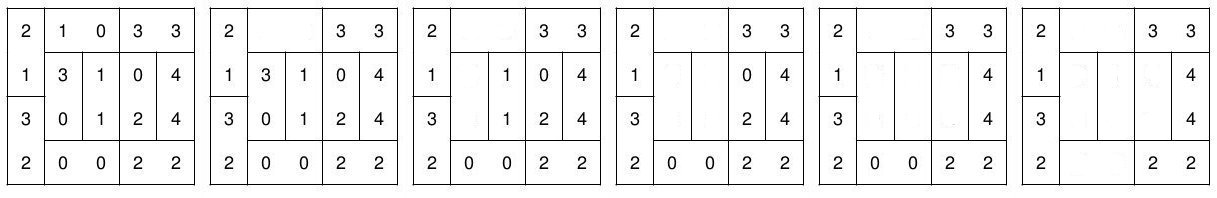
\includegraphics[width=1\textwidth]{board1.jpg} \\
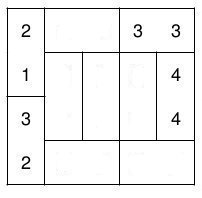
\includegraphics[width=0.163\textwidth]{board2.jpg}

\end{document}
